\documentclass{beamer}
\usepackage{csquotes}
\usepackage{tikz}
\usetikzlibrary{arrows,positioning,shapes.geometric, calc}
\usepackage{amsmath}
\usepackage{listings, xcolor}
\usepackage{lmodern}
\usepackage{adjustbox}
\usepackage{booktabs}
\usepackage{colortbl}
\usepackage{caption}
\usepackage{icomma}
\usepackage{bigstrut}
\usepackage{geometry}
\usepackage{subfigure}
\usepackage{algorithmic}


\DeclareMathOperator*{\argmin}{argmin}
\captionsetup[figure]{labelformat=empty}

\usetheme{metropolis}           % Use metropolis theme
\title{Update: NN project}
\date{\today}
\author{Robert M. Porsch}
\institute{Center for Genomic Science}
\begin{document}
\maketitle

\begin{frame}[t]{Training, Development, Testing}
  \begin{columns}[t]
    \begin{column}{0.5\textwidth}
      Simulation Data 1:\\
      \begin{itemize}
        \item $\sim2,000$ samples
        \item 40 different simulated phenotypes
        \item based on 1000 Genome project
        \item $MAF\geq1\%$
      \end{itemize}
    \end{column}
    \begin{column}{0.5\textwidth}
     Simulation Data 2: 
     \begin{itemize}
       \item $\sim300,000$ samples
       \item 4 different simulated phenotypes
       \item based on UKB
        \item $MAF\geq1\%$
     \end{itemize}
    \end{column}
  \end{columns}
  Issues: sample size limitations for development/testing dataset 
\end{frame}

\begin{frame}[t]{On the issue of clumping}
  \begin{itemize}
    \item Clumping can be seen as a variable selection methods (with the parameter p1, p2, r2 and window size)
    \item Tests for a linear relationship between SNP and phenotype
  \end{itemize}
  So when is this becoming a problem?
  \begin{itemize}
    \item nonlinearity
    \item interactions
    \item additional hypterparameter to optimize
  \end{itemize}
\end{frame}

\begin{frame}[t]{On the sucess of clumping}
  \begin{columns}
    \begin{column}{0.5\textwidth}
      \begin{figure}[htpb]
        \centering
        \includegraphics[width=0.8\linewidth]{./clumped_1kg_lasso.png}
        \caption{Clumped Lassosum}
      \end{figure}
    \end{column}
    \begin{column}{0.5\textwidth}
      \begin{figure}[htpb]
        \centering
        \includegraphics[width=0.8\linewidth]{./not_clumped_1kg_lasso.png}
        \caption{NOT Clumped Lassosum}
      \end{figure}
    \end{column}
  \end{columns}
\end{frame}

\begin{frame}[t]{NN are difficult to fit}
  \begin{columns}
    \begin{column}{0.5\textwidth}
      \begin{figure}[htpb]
        \centering
        \includegraphics[width=0.8\linewidth]{keras_model_ukb_nn}
        \caption{Complex model (85,60,60,60)}
      \end{figure}
    \end{column}
    \begin{column}{0.5\textwidth}
      \begin{figure}[htpb]
        \centering
        \includegraphics[width=0.8\linewidth]{keras_model_ukb_nn_small}
        \caption{Simple model (60)}
      \end{figure}
    \end{column}
  \end{columns}
  \begin{itemize}
    \item Complexity becomes difficult to train (learning rate)
    \item The phenotype is linear
  \end{itemize}
\end{frame}

\begin{frame}[t]{Sometimes you need to think}
  \begin{columns}
    \begin{column}{0.5\textwidth}
      \begin{figure}[htpb]
        \centering
        \includegraphics[width=0.8\linewidth]{keras_model_ukb_linear.png}
        \caption{Linear Model on the UKB}
      \end{figure}
    \end{column}
    \begin{column}{0.5\textwidth}
      \begin{figure}[htpb]
        \centering
        \includegraphics[width=0.8\linewidth]{./keras_model_ukb_nn_small.png}
        \caption{Small NN model on the UKB}
      \end{figure}
    \end{column}
  \end{columns}
  \begin{itemize}
    \item Drop out layer regularizes efficiently
    \item During validation dropout is deactivated
  \end{itemize}
\end{frame}

\begin{frame}[t]{On Sample Size}
  \begin{columns}
    \begin{column}{0.5\textwidth}
      \begin{figure}[htpb]
        \centering
        \includegraphics[width=0.8\linewidth]{./keras_model_ukb_nn_small.png}
        \caption{Small NN model on the UKB}
      \end{figure}
    \end{column}
    \begin{column}{0.5\textwidth}
      \begin{figure}[htpb]
        \centering
        \includegraphics[width=0.8\linewidth]{./keras_model_1kg_nn_small.png}
        \caption{Small NN model on the 1KG}
      \end{figure}
    \end{column}
  \end{columns}
  \begin{itemize}
    \item less overfitting
    \item results remain accurate despite low sample size
  \end{itemize}
\end{frame}

\begin{frame}[t]{Evaluation}
  \begin{itemize}
    \item Trivial problem given a linear simulated phenotype
    \item Now-complexity
  \end{itemize}
\end{frame}

% \begin{frame}[t]{UKB Data}
%   I also made use of the UKB with the following phenotypes:
%   \begin{itemize}
%     \item height
%     \item IQ
%   \end{itemize}
%   Data was split into training and dev set using caucsian samples only.
%   Dev set was set to be at least $10,000$ samples.
% 
%   Some potential problems with the data structure:
%   \begin{itemize}
%     \item data was not shuffled 
%     \item currently data was not adjusted for potential confounders (unclear how important)
%   \end{itemize}
% \end{frame}
% 
% \section{Fully connected LD Layer: FullDa}
% 
% \begin{frame}[t]{Architecture}
%   \begin{columns}[t]
%     \begin{column}{0.5\textwidth}
%       Layer 1:
%       \begin{algorithmic}
%         \STATE initialize $Z$
%         \FOR{v = LD-Blocks} 
%         \STATE $z_v = W^{[1]}_vX_v$
%         \STATE $a_v = g(z_v)$
%         \STATE $APPEND(Z, z_v)$
%         \ENDFOR
%       \end{algorithmic}
%       Layer $2$:\\
%       \begin{itemize}
%         \item fully connected layers to output
%         \item $L_1$ regularization in $l=1,2$
%         \item dropout with $p=0.8$
%       \end{itemize}
%     \end{column}
%     \begin{column}{0.5\textwidth}
%       Optimization:
%       \begin{itemize}
%         \item AdaGrad
%         \item Mini-Batch gradient decent with $m=100$
%         \item no early stopping ($epochs=100$)
%       \end{itemize}
%     \end{column}
%   \end{columns}
% \end{frame}
% 
% \begin{frame}[t]{Model Overview}
%   \begin{figure}[htpb]
%     \centering
%     \includegraphics[width=0.8\linewidth]{./tensormodel.png}
%   \end{figure}
% \end{frame}
% 
% \begin{frame}[t]{Some results}
%   \begin{figure}[htpb]
%     \centering
%     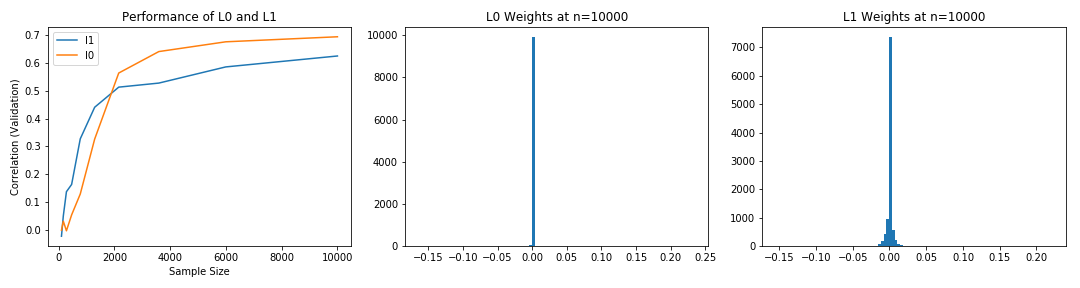
\includegraphics[width=0.8\linewidth]{performance.png}
%     \caption{Example performance on phenotype 1}
%   \end{figure}
%   \begin{itemize}
%     \item high variance problem
%     \item disappointing performance in development set
%     \item performance similar to LassoSum
%   \end{itemize}
% \end{frame}
% 
% \section{Clumped NN}
% 
% \begin{frame}[t]{Architecture}
%   Similar architecture but with additional clumping step
% 
%   \begin{enumerate}[(i)]
%     \item run GWAS on training set
%     \item perform clumping ($r^2=0.5, p_1 = 0.01, p_2 = 0.1$) 
%       \begin{itemize}
%         \item Results in 72 SNPs
%       \end{itemize}
%     \item feed clumped genotype matrix into fully connected NN $L=3$
%       \begin{itemize}
%         \item $n^{[1]}_h=60, n^{[2]}_h=60, n^{[3]}_h=1$
%         \item dropout layer after $l=1$ and $l=2$
%       \end{itemize}
%   \end{enumerate}
%   No early stopping, ($epochs=100$), mini-batch with $m=100$
% \end{frame}
% 
% \begin{frame}[t]{Results}
%   \begin{figure}[htpb]
%     \centering
%     \includegraphics[width=0.8\linewidth]{./keras_model.png}
%   \end{figure}
%   \begin{itemize}
%     \item Similar performance to the LD-connected NN
%     \item high variance problem
%   \end{itemize}
% \end{frame}
% 
% \begin{frame}[t]{Conclusions}
%   \begin{itemize}
%     \item Stronger regularization is required
%     \item Currently there is no hyper-parameter optimization
%     \item Larger dataset should be used (requires some re-write of the data import)
%     \item Current literature: More and more paper on penalized regression for genetic risk prediction (mostly Lasso)
%   \end{itemize}
% \end{frame}
\end{document}
